\documentclass[border=5pt]{standalone}
\usepackage{tikz}
\usetikzlibrary{shapes.geometric, arrows}

% These are templates for each block
\tikzstyle{startstop} = [rectangle, rounded corners, minimum width=3cm, minimum height=1cm,text centered, draw=black, fill=red!30]

\tikzstyle{io} = [trapezium, trapezium left angle=70, trapezium right angle=110, minimum width=3cm, minimum height=1cm,text width=3cm,, text centered, draw=black, fill=blue!30]

\tikzstyle{process} = [rectangle, minimum width=3cm, minimum height=1cm, text centered, text width=3cm, draw=black, fill=orange!30]

\tikzstyle{arrow} = [thick,->,>=stealth]

\tikzstyle{decision} = [diamond, minimum width=3cm, minimum height=1cm, text centered, draw=black, fill=green!30]

\begin{document}
% custom unit vector lengths, each node is spaced by 2cm
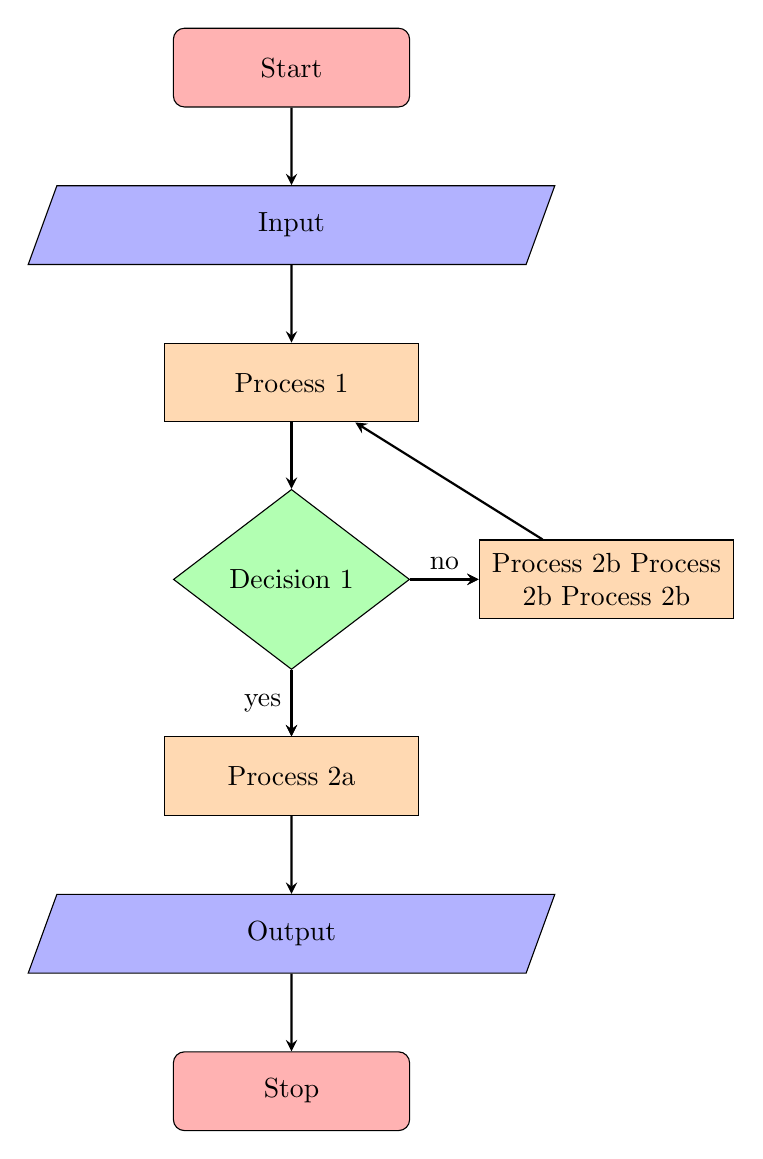
\begin{tikzpicture}[x=1cm,y=1cm, node distance=2cm]
%%%%% ADDING MAIN BLOCKS


% \node (node name) [options] {node content};
%(node name) is an optional identifier for the node and can be used to refer to it later, for drawing lines or positioning other nodes relative to it.
%[options] are the settings for the node, such as its shape, style, color, etc.
%{node content} is the text or the content that appears inside the node.
\node (start) [startstop] {Start}; %startstop defined earlier
% We could also use above of, right of or left of if we wanted the block to appear somewhere else. 
\node (in1) [io, below of=start] {Input};
\node (pro1) [process, below of=in1] {Process 1};
%\node (dec1) [decision, below of=pro1] {Decision 1};
 % we can manually shift these boxes if needed
\node (dec1) [decision, below of=pro1, yshift=-0.5cm] {Decision 1};
\node (pro2a) [process, below of=dec1, yshift=-0.5cm] {Process 2a};
\node (pro2b) [process, right of=dec1, xshift=2cm] {Process 2b Process 2b Process 2b };
\node (out1) [io, below of=pro2a] {Output};
\node (stop) [startstop, below of=out1] {Stop};

%%%%% ADDING ARROWS
\draw [arrow] (start) -- (in1);
\draw [arrow] (in1) -- (pro1);
\draw [arrow] (pro1) -- (dec1);
\draw [arrow] (dec1) -- (pro2a);
\draw [arrow] (dec1) -- (pro2b);

\draw [arrow] (dec1) -- node[anchor=east] {yes} (pro2a);
\draw [arrow] (dec1) -- node[anchor=south] {no} (pro2b);

\draw [arrow] (pro2b) -- (pro1);
\draw [arrow] (pro2a) -- (out1);
\draw [arrow] (out1) -- (stop);
\end{tikzpicture}
\end{document}